\documentclass{article}
\usepackage{tikz}
\begin{document}

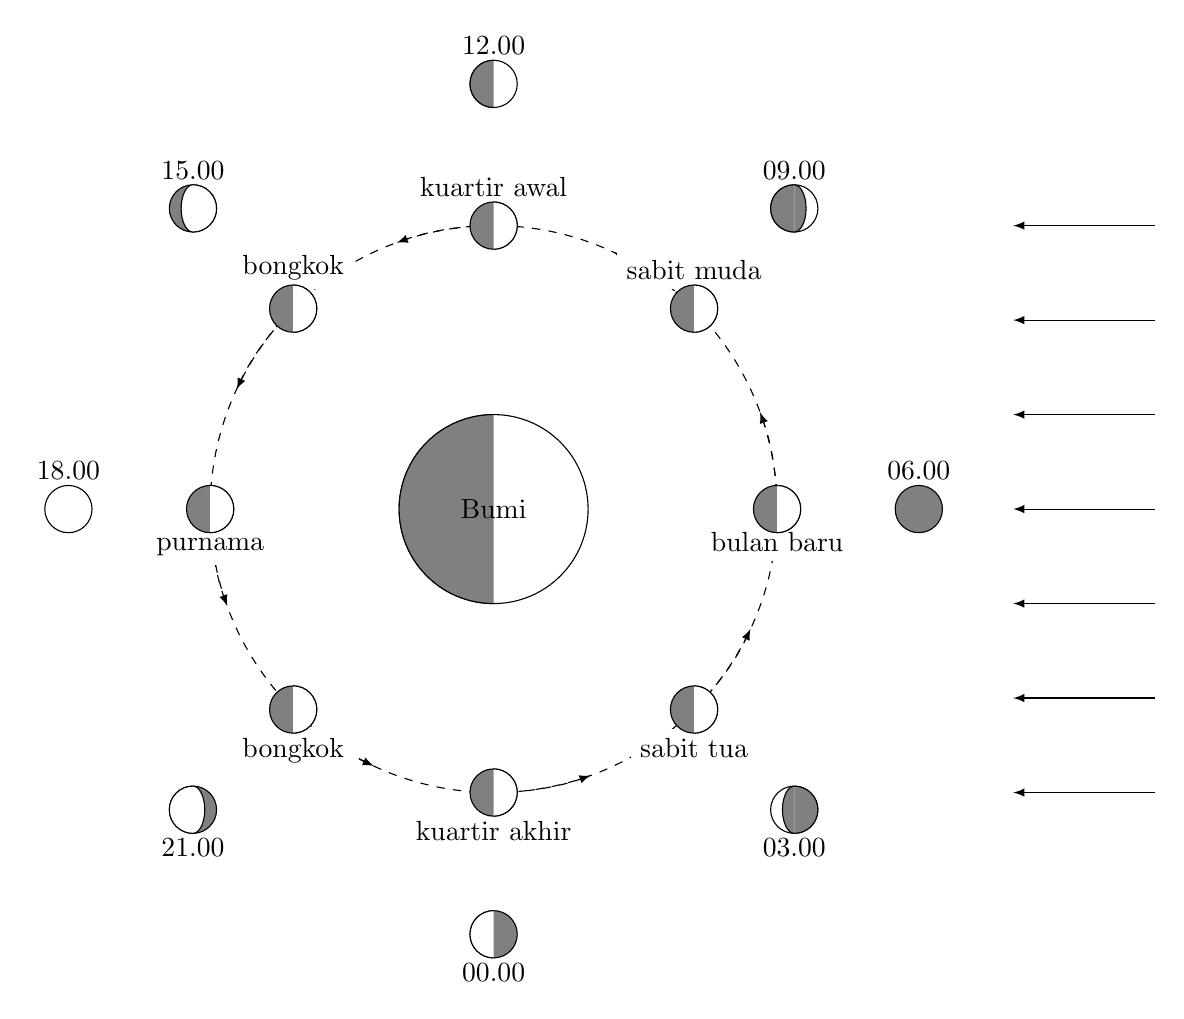
\begin{tikzpicture}[>=latex, scale=1.2]
\draw (0,0) circle (1);
\draw [dashed] (0,0) circle (3);

\draw (0,1) [fill=gray] arc (90:270:1);
\draw (0,0) node {Bumi};

\foreach \x in {0,45,...,315}{
	\draw (\x:3) [->,dashed] arc (\x:\x+20:3);
}

\tikzstyle{every node}=[fill=white]
\draw (0:3) node [below=5] {bulan baru};
\draw (45:3) node [above=7] {sabit muda};
\draw (90:3) node [above=7] {kuartir awal};
\draw (135:3) node [above=7] {bongkok};
\draw (180:3) node [below=7] {purnama};
\draw (225:3) node [below=7] {bongkok};
\draw (270:3) node [below=7] {kuartir akhir};
\draw (315:3) node [below=7] {sabit tua};

\draw (0:4.5) node [above=7] {06.00};
\draw (45:4.5) node [above=7] {09.00};
\draw (90:4.5) node [above=7] {12.00};
\draw (135:4.5) node [above=7] {15.00};
\draw (180:4.5) node [above=7] {18.00};
\draw (225:4.5) node [below=7] {21.00};
\draw (270:4.5) node [below=7] {00.00};
\draw (315:4.5) node [below=7] {03.00};

\draw (0:4.5) [fill=gray] circle (0.25);
\draw (45:4.5) [fill=white] circle (0.25);
	\draw (45:4.5)+(0,-0.25) [fill=gray] arc (-90:90:0.125 and 0.25);
	\draw (45:4.5)+(0,0.25) [fill=gray] arc (90:270:0.25 and 0.25);
\draw (90:4.5) [fill=white] circle (0.25);
	\draw (90:4.5)+(0,0.25) [fill=gray] arc (90:270:0.25 and 0.25);
\draw (135:4.5) [fill=gray] circle (0.25);
	\draw (135:4.5)+(0,0.25) [fill=white] arc (90:270:0.125 and 0.25);
	\draw (135:4.5)+(0,-0.25) [fill=white] arc (-90:90:0.25 and 0.25);
\draw (180:4.5) [fill=white] circle (0.25);
\draw (225:4.5) [fill=gray] circle (0.25);
	\draw (225:4.5)+(0,-0.25) [fill=white] arc (-90:90:0.125 and 0.25);
	\draw (225:4.5)+(0,0.25) [fill=white] arc (90:270:0.25 and 0.25);
\draw (270:4.5) [fill=gray] circle (0.25);
	\draw (270:4.5)+(0,0.25) [fill=white] arc (90:270:0.25 and 0.25);
\draw (315:4.5) [fill=white] circle (0.25);
	\draw (315:4.5)+(0,0.25) [fill=gray] arc (90:270:0.125 and 0.25);
	\draw (315:4.5)+(0,-0.25) [fill=gray] arc (-90:90:0.25 and 0.25);

\foreach \x in {0,45,...,315}{
	\draw (\x:3) [fill=gray] circle (0.25);
	\draw (\x:3)+(0,-0.25) [fill=white] arc (-90:90:0.25);
}

\foreach \x in {-3,-2,...,3} \draw [->] (7,\x) -- +(-1.5,0);

\end{tikzpicture}
\end{document}